\documentclass[conference]{IEEEtran}

\usepackage{cite}
\usepackage{amsmath,amssymb,amsfonts}
\usepackage{algorithmic}
\usepackage{graphicx}
\usepackage{textcomp}
\usepackage{xcolor}
\usepackage{hyperref}
\def\BibTeX{{\rm B\kern-.05em{\sc i\kern-.025em b}\kern-.08em
    T\kern-.1667em\lower.7ex\hbox{E}\kern-.125emX}}

\hypersetup{
	colorlinks=true,
	linkcolor=black,
	filecolor=black,      
	urlcolor=black,
	citecolor=black
}
\begin{document}

\title{Evaluating Matrix Factorization Robustness in Highly Sparse Movie Recommendation Datasets}

\author{\IEEEauthorblockN{Gabriel Guillen}
\IEEEauthorblockA{\textit{dept. of Statistics \& Data Science} \\
\textit{University of Central Florida}\\
Orlando, United States of America \\
ga013701@ucf.edu}}


\maketitle
\renewcommand{\abstractname}{Summary}
\begin{abstract}
	This study evaluates three matrix factorization models---\textbf{Funk Singular Value Decomposition (Funk SVD)}, \textbf{Latent Factor Models (LFM-SGD)}, and \textbf{Sparse Coding}---for movie recommendation. Models were validated using RMSE and other regression-based metrics to assess prediction accuracy, alongside ranking metrics to evaluate recommendation quality. Experimental results indicate that \textbf{Sparse Coding} consistently outperforms the alternative techniques across all metrics, showing it is better at predicting ratings and works more reliably on new, unseen data.
\end{abstract}

\section{\textbf{Introduction}}\indent Matrix factorization is essential for mitigating missing data effects in recommendation systems. This study compares three models: \textbf{Funk Singular Value Decomposition (Funk SVD)}, \textbf{Latent Factor Models (LFM-SGD)}, and \textbf{Sparse Coding}.\\
\indent The primary objective is to predict user ratings despite the extreme sparsity of interactions. We leverage dimensionality reduction to map users and items into a shared latent space, and handling the problem of missing information. Performance is evaluated via \textbf{RMSE}, \textbf{MAE}, \textbf{Precision}, \textbf{Recall}, and \textbf{NDCG}.\\
\indent While SVD and LFM-SGD are benchmarks, we hypothesize that \textbf{Sparse Coding} is better suited for sparse data. By using an overcomplete dictionary and regularization, it focuses on the most important data and ignores errors, capturing subtle preferences that traditional global-variance methods may overlook.
\indent While traditional methods provide a baseline, this study focuses on the comparative resilience of Sparse Coding when dealing with a dataset where 93.7\% of the ratings are missing.

\subsection{\textbf{Dataset Structure}}
\indent This study utilizes the \textbf{MovieLens 100K}\cite{harper2015movielens} dataset, which consists of 100,000 ratings ($R \in \{1, 2, 3, 4, 5\}$) provided by 943 users across 1,682 movies. The dataset exhibits a sparsity common in recommendation tasks, with a density of 6.304\%.\\ 
\indent The data is partitioned into training and testing subsets to facilitate model validation. Each observation is structured in a four-column format: \texttt{'user item rating timestamp'}.\\ 
\indent Auditing of the entries confirmed a clean feature space, allowing for direct mapping of user-item interactions into the latent factor models.

\vspace{4mm}

\section{\textbf{Methods}}

\subsection{\textbf{Model Preparation}}

The models were trained on a sparse \textbf{User-Item interaction matrix} \cite{harper2015movielens} of 943 users ($U$) and 1,682 movies ($I$). Using pre-partitioned subsets, the models learned latent factors to predict ratings that were kept hidden during training.

\vspace{2mm}

\subsection{\textbf{Performance Evaluation}}
To identify which model best captures subtle preferences in sparse data, performance was measured using several predictive and ranking metrics. Alongside \textbf{Mean Absolute Error (MAE)} \cite{ISLR2}, the primary error metric was \textbf{Root Mean Square Error (RMSE)} \cite{harper2015movielens}:

\begin{equation}
	RMSE = \sqrt{\frac{\sum_{u \in U, i \in I} (R_{ui} - R'_{ui})^2}{Number \ of \ Ratings}}
\end{equation} 
Where $R_{ui}$ and $R'_{ui}$ represent the actual and predicted ratings for user $u$ and item $i$, respectively. 

We complement RMSE with \textbf{Normalized Discounted Cumulative Gain (NDCG)}\cite{Jarvelin2002} to evaluate ranking quality, using logarithmic decay to reward models that surface relevant items.\\ 
\indent To further assess relevance, \textbf{Precision}\cite{ISLR2} and \textbf{Recall}\cite{ISLR2} were calculated using a threshold of 3, where ratings $\ge 3$ are classified as ``good'' and others as irrelevant.\\
\indent This multi-metric approach provides a robust benchmark framework.

\vspace{2mm}

\subsection{\textbf{Matrix Factorization Models Used}}

\begin{enumerate}
	\item \textbf{Funk Singular Value Decomposition (Funk SVD)} \cite{funk2006}: A latent factor benchmark that factorizes the user-item matrix by optimizing solely over observed ratings via SGD. Configured with 50 latent factors ($k=50$), a learning rate ($\eta = 0.005$), and regularization ($\lambda = 0.02$) over 50 epochs, it extracts latent features without the bias of dense imputation.
		
	\item \textbf{Latent Factor Models (LFM-SGD)} \cite{koren2009}: A model utilizing Stochastic Gradient Descent to learn user/item embeddings ($k=20$ latent factors, 20 iterations). By optimizing only over observed entries, it scales efficiently to sparse matrices and captures nuanced patterns without requiring data imputation.
	
	\item \textbf{Sparse Coding} \cite{olshausen1996}: A generative framework that represents data as a sparse linear combination of atoms from an overcomplete dictionary. Utilizing Elastic Net regularization (with $\lambda = 0.01, \alpha = 0.01$), it isolates salient features by activating only the most relevant basis functions, effectively filtering noise.
\end{enumerate}

\vspace{6mm}

\section{\textbf{Experimental Results and Metric Divergence}}

The experimental results as shown in Figure \ref{graph_radar_profile} indicate a a big difference between a model's ability to rank movies correctly and its ability to guess the exact rating. While \textbf{Sparse Coding} achieves a near-optimal \textbf{NDCG of 0.99}, its \textbf{Norm\_Accuracy} remains low at \textbf{0.13}.\\

\begin{figure}[htbp]
	\centerline{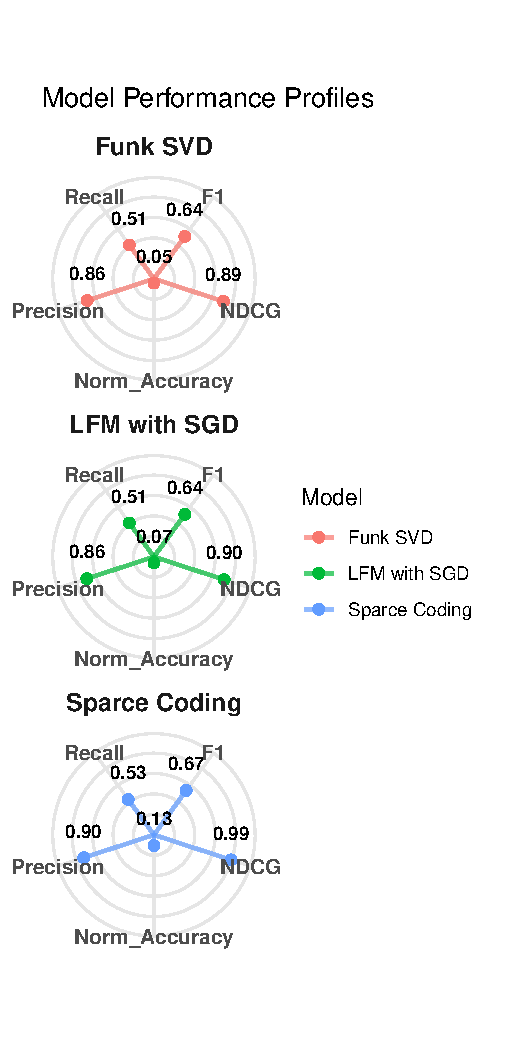
\includegraphics[scale=0.75]{radar_profile.pdf}}
	\caption{Models Profile By Measuring Metrics}
	\label{graph_radar_profile}
\end{figure}

\indent This divergence suggests that the model effectively captures relative preference hierarchies (ranking) despite high absolute error in point-wise rating prediction ($Norm\_Accuracy = 1 - RMSE_{test}$).

Similarly, \textbf{LFM-SGD} and \textbf{Funk SVD} demonstrate robust ranking capabilities with \textbf{NDCG} values of \textbf{0.90} and \textbf{0.89} respectively, yet yield negligible \textbf{Norm\_Accuracy} scores ($\le 0.07$).\\
\indent This gap shows that while models understand which movies a user likes more than others, they struggle to hit adequate \textbf{RMSE}.\\ 
\indent Consequently, these models are highly effective for recommendation retrieval where item ordering is prioritized over exact rating accuracy.

\vspace{6mm}

\section{\textbf{Discussion}}

\subsection{\textbf{Comparative Model Performance}}

The performance analysis in Figure \ref{graph_error_comparison} reveals a consistent trend in generalization, with test error remaining comparable to training error across all models.\\
\indent This stability suggests that underlying patterns were captured without significant overfitting; however, the \textbf{persistent magnitude of the RMSE} indicates that the models have reached a predictive floor.

\begin{figure}[htbp]
	\centerline{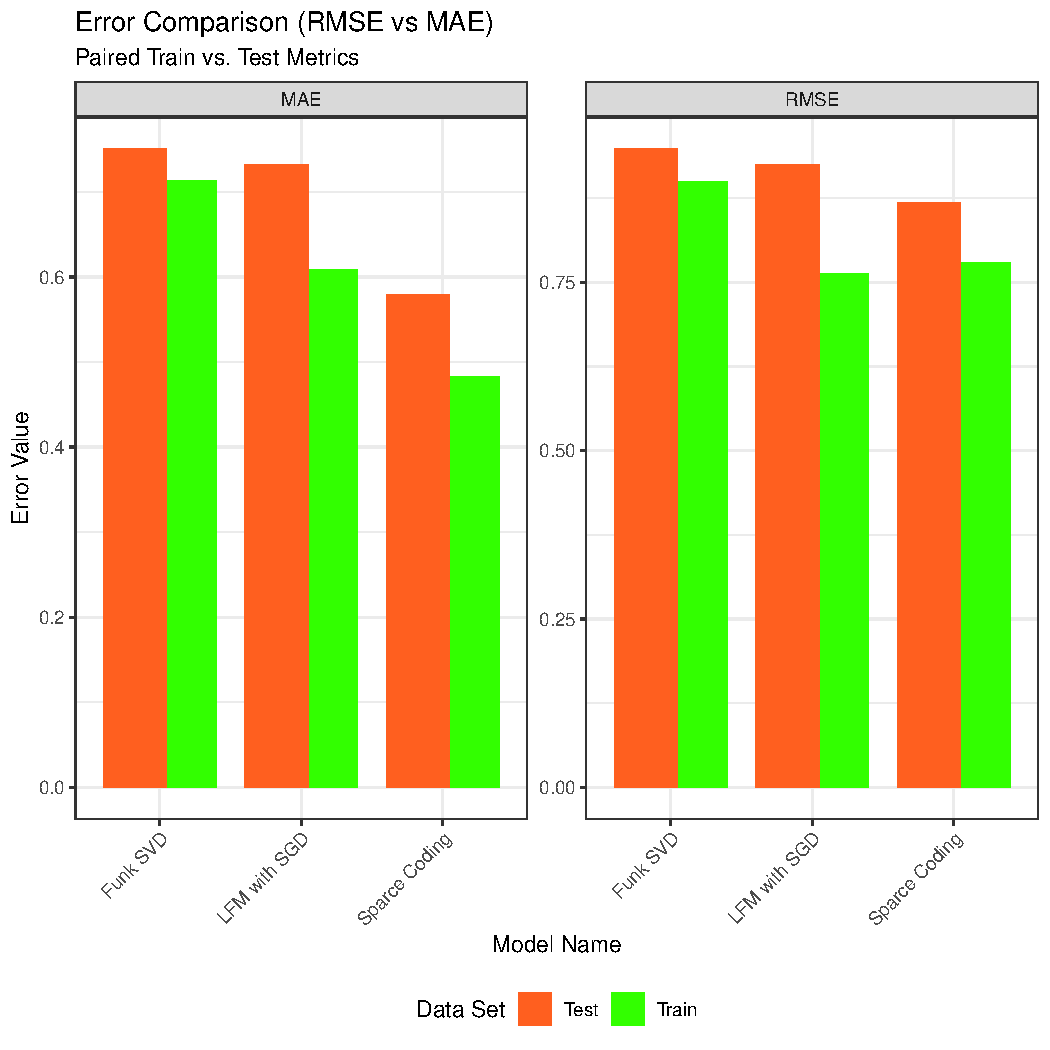
\includegraphics[scale=0.60]{error_comparison.pdf}}
	\caption{Error Comparison by Model}
	\label{graph_error_comparison}
\end{figure} 

Sparse Coding demonstrates the highest efficiency, achieving the lowest MAE and RMSE values. Its superior training and test results indicate it is the most capable model for mapping user features to ratings.

In contrast, \textbf{LFM-SGD} and \textbf{Funk SVD} exhibit higher baseline error rates. While their training and test metrics are closely aligned, their higher values indicate less precision in predicting exact ratings compared to \textbf{Sparse Coding}.

\subsection{\textbf{Model Generalization}}

Observing the slope graph in Figure \ref{graph_ndcg_slope} \textbf{Sparse Coding} achieved the highest performance, maintaining a stable \text{NDCG} of approximately $0.99$ across both training and testing datasets. This minimal variance indicates exceptional generalization and high accuracy on unseen data.

 \begin{figure}[htbp]
	\centerline{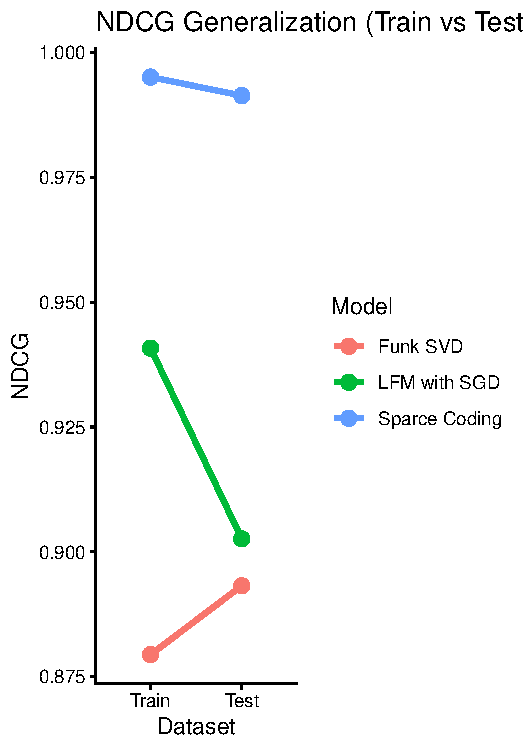
\includegraphics[scale=1]{ndcg_slope.pdf}}
	\caption{NDCG by Model}
	\label{graph_ndcg_slope}
\end{figure}

\textbf{Funk SVD} exhibited a unique upward trend, with its \text{NDCG} rising from $0.88$ during training to $0.89$ in the testing phase. This slight improvement suggests the model is highly robust and effectively avoids overfitting.

\textbf{LFM-SGD} proved to be the weakest model in generalization. Its \text{NDCG} dropped sharply from $0.94$ on the training set to below $0.90$ on the test set.\\
\indent This significant decline represents the largest generalization gap in the analysis, indicating substantial overfitting.

\newpage

\subsection{\textbf{Evaluating Model Recommendation Efficacy}}

The visualization highlights shown in Figure \ref{graph_precision_vs_cecall} the trade-off between \textbf{Precision (the quality of recommendations)} and \textbf{Recall (the breadth of recommendations)}.\\
\indent \textbf{Sparse Coding} emerges as the superior model, occupying the top-right position with a \textbf{Precision} $\approx 0.90$ and \textbf{Recall} $\approx 0.54$, effectively maximizing relevance while minimizing noise.

\begin{figure}[htbp]
	\centerline{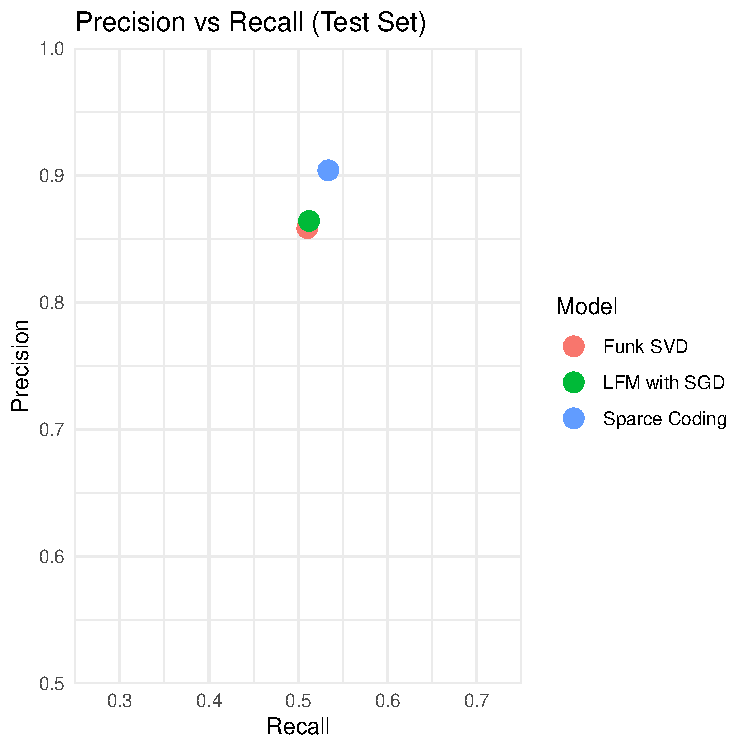
\includegraphics[scale=.80]{pr_scatter.pdf}}
	\caption{Precision-Recall Comparison Among Models}
	\label{graph_precision_vs_cecall}
\end{figure}

\textbf{LFM-SGD} occupies the middle tier, yielding a \textbf{Precision} $\approx 0.86$ and \textbf{Recall} $\approx 0.51$.\\
\indent Finally, \textbf{Funk SVD} is the least performant model, sitting at the base of the cluster with a \textbf{Precision} of 0.85 and the lowest \textbf{Recall} at 0.50, capturing the smallest portion of relevant items.

\vspace{10mm}

\section{\textbf{Conclusion}}

This study evaluated three matrix factorization models---\textbf{Funk SVD}, \textbf{LFM-SGD}, and \textbf{Sparse Coding}---on the MovieLens 100K dataset.\\
\indent Despite the 93.7\% sparsity and the complexity of the \textbf{latent factor space}, \textbf{Sparse Coding} emerged as the most robust framework, achieving superior precision and generalization.

A critical finding is the divergence between error-based and ranking-based metrics. While \textbf{RMSE} measures point-wise prediction magnitude, it proved insufficient as a sole indicator of quality. Even as models reached a ``predictive floor'' in absolute accuracy, their ranking proficiency remained high.

The inclusion of \textbf{NDCG} was essential for this evaluation. While \textbf{RMSE} quantifies distance from actual values, \textbf{NDCG} rewards the correct ordering of recommendation lists.\\
\indent \textbf{Sparse Coding} achieved a near-perfect \textbf{NDCG} of 0.99, demonstrating that it effectively find and recommend the right movies even when absolute predictions contain noise. 

For real-world systems, where "top-$N$" accuracy is paramount, ranking proficiency is a more vital indicator of user satisfaction than \textbf{RMSE}.\\
\indent The superior performance of \textbf{Sparse Coding} across \textbf{Precision-Recall}, \textbf{NDCG}, and \textbf{RMSE}---relative to both \textbf{Funk SVD} and \textbf{LFM-SGD}---confirms its enhanced ability to isolate salient features within sparse matrices.\\
\indent Because \textbf{Sparse Coding} achieves high NDCG and Precision, it ensures that the 'highest predicted ratings' generated by the model truly correspond to the items the user is most likely to enjoy.

\begin{thebibliography}{9} % '9' is for formatting the numbering (up to 9 items)
	
\bibitem{harper2015movielens}
Harper, F. M., and Konstan, J. A. (2015). 
\newblock The MovieLens datasets: History and context. 
\newblock \textit{ACM Transactions on Interactive Intelligent Systems (TiiS)}, 5(4), 1--19.
\newblock \url{https://doi.org/10.1145/2827872}

\bibitem{paperswithcode_movielens}
Papers with Code. (2026).
\newblock Collaborative Filtering on MovieLens 100K.
\newblock \url{https://paperswithcode.com/sota/collaborative-filtering-on-movielens-100k}

\bibitem{funk2006}
S.~Funk.
\newblock Netflix Update: Try This at Home.
\newblock \url{http://sifter.org/~simon/journal/20061211.html}, 2006.
\newblock Accessed: May 20, 2024.

\bibitem{koren2009}
Koren, Y., Bell, R., and Volinsky, C. (2009). 
\newblock Matrix factorization techniques for recommender systems. 
\newblock \textit{Computer}, 42(8), 30--37.

\bibitem{olshausen1996}
Olshausen, B. A., and Field, D. J. (1996). 
\newblock Emergence of simple-cell receptive field properties by learning a sparse code for natural images. 
\newblock \textit{Nature}, 381(6583), 607--609.

\bibitem{ISLR2} 
James, G., Witten, D., Hastie, T., and Tibshirani, R. (2021). 
\textit{An Introduction to Statistical Learning: with Applications in R} (2nd ed.). 
Springer Texts in Statistics. New York: Springer.

\bibitem{Jarvelin2002} 
Järvelin, K., and Kekäläinen, J. (2002). 
\textit{Cumulated gain-based evaluation of IR techniques}. 
ACM Transactions on Information Systems (TOIS), 20(4), 422–446. 
https://doi.org/10.1145/582415.582418

\section*{\textbf{Appendix}}

\section*{Appendix A: Supplementary Materials and Software Usage}
\subsection*{Source Code Repository \label{app:code}}
The source code, data, and detailed implementation scripts for this project are available on GitHub (URL: \url{https://github.com/gaguillen4384-dev/Data-Science/tree/main/DataMining_2/Movie_Recommender_Model_Analysis}).

\subsection*{Software Usage Acknowledgment}
\begin{enumerate}
	\item The text and documentation were edited and refined using \textbf{Google Gemini}.
	\item \textbf{R} (version 4.x.x) was used for model computation and graphics development.
	\item The following \textbf{R} libraries were essential to the computational workflow:
	\begin{itemize}
		\item \textbf{recosystem}: Utilized for Latent Factor Modeling via Stochastic Gradient Descent (LFM-SGD).
		\item \textbf{glmnet}: Applied for Sparse Coding through regularized generalized linear models.
		\item \textbf{Matrix}: Used to manage and manipulate sparse matrix structures required for high-dimensional computations.
		\item \textbf{jsonlite}: Employed for the robust parsing and processing of JSON-formatted data.
		\item \textbf{dplyr} \& \textbf{tidyr}: Used for data manipulation, cleaning, and reshaping into tidy formats.
		\item \textbf{ggplot2}: Used for the development of all statistical graphics and data visualizations.
	\end{itemize}
\end{enumerate}

	
\end{thebibliography}

\vspace{12pt}

\end{document}
